
%(BEGIN_QUESTION)
% Copyright 2013, Tony R. Kuphaldt, released under the Creative Commons Attribution License (v 1.0)
% This means you may do almost anything with this work of mine, so long as you give me proper credit

Suppose you are asked to configure the instruments in this temperature control loop to sense and display process temperature over a range of 200 to 1800 degrees Celsius, with the loop controller actuating two split-ranged control valves in a complementary sequence:

$$\includegraphics[width=15.5cm]{i02078x01.eps}$$

Write the proper range values inside the boxes near each instrument, showing the proper configuration for each instrument needed to achieve the desired result.

\vskip 20pt \vbox{\hrule \hbox{\strut \vrule{} {\bf Suggestions for Socratic discussion} \vrule} \hrule}

\begin{itemize}
\item{} Suppose the controller displayed a temperature of 1246 when the actual process temperature was 1265 $^{o}$C.  First, identify {\it two} possible locations in this loop for a calibration error that would account for this discrepancy.  Then, assuming only one fault, explain how you could positively determine the location of this calibration error with a single diagnostic test.
\item{} Suppose valve TV-A was 44\% open and TV-B was 56\% open when the controller output displayed 52\%.  First, identify {\it two} possible locations in this loop for a calibration error that would account for this discrepancy.  Then, assuming only one fault, explain how you could positively determine the location of this calibration error with a single diagnostic test.
\end{itemize}

\underbar{file i02078}
%(END_QUESTION)





%(BEGIN_ANSWER)

$$\includegraphics[width=15.5cm]{i02078x02.eps}$$

%(END_ANSWER)





%(BEGIN_NOTES)

A PV measurement error could lie within the transmitter, or within the controller's analog input.  A single current measurement of the transmitter's signal will tell you where the calibration error resides.

\vskip 10pt

A valve positioning error affecting both control valves could lie within the I/P transducer or within the controller's analog output.  A single current measurement of the controller's output signal will tell you where the calibration error resides.

%INDEX% Basics, transmitter: input and output ranges
%INDEX% Final Control Elements, valve: split ranging

%(END_NOTES)

